\newpage
\subsection{Ký số tập tin}

\subsubsection*{Mục tiêu}
Chức năng ký số cho phép người dùng xác minh tính \textbf{toàn vẹn} và \textbf{nguồn gốc xác thực} của tập tin. Người gửi sử dụng private key RSA để ký tập tin, từ đó sinh ra một file chữ ký \texttt{.sig}. Người nhận có thể xác minh bằng public key tương ứng.

\subsubsection*{Giao diện}
Giao diện \texttt{/utils/sign\_file} cho phép:
\begin{itemize}
    \item Chọn file bất kỳ để ký
    \item Submit và tải về file chữ ký \texttt{.sig}
    \item Hiển thị thông báo (toast) khi ký thành công hoặc lỗi
\end{itemize}

\begin{figure}[H]
    \centering
    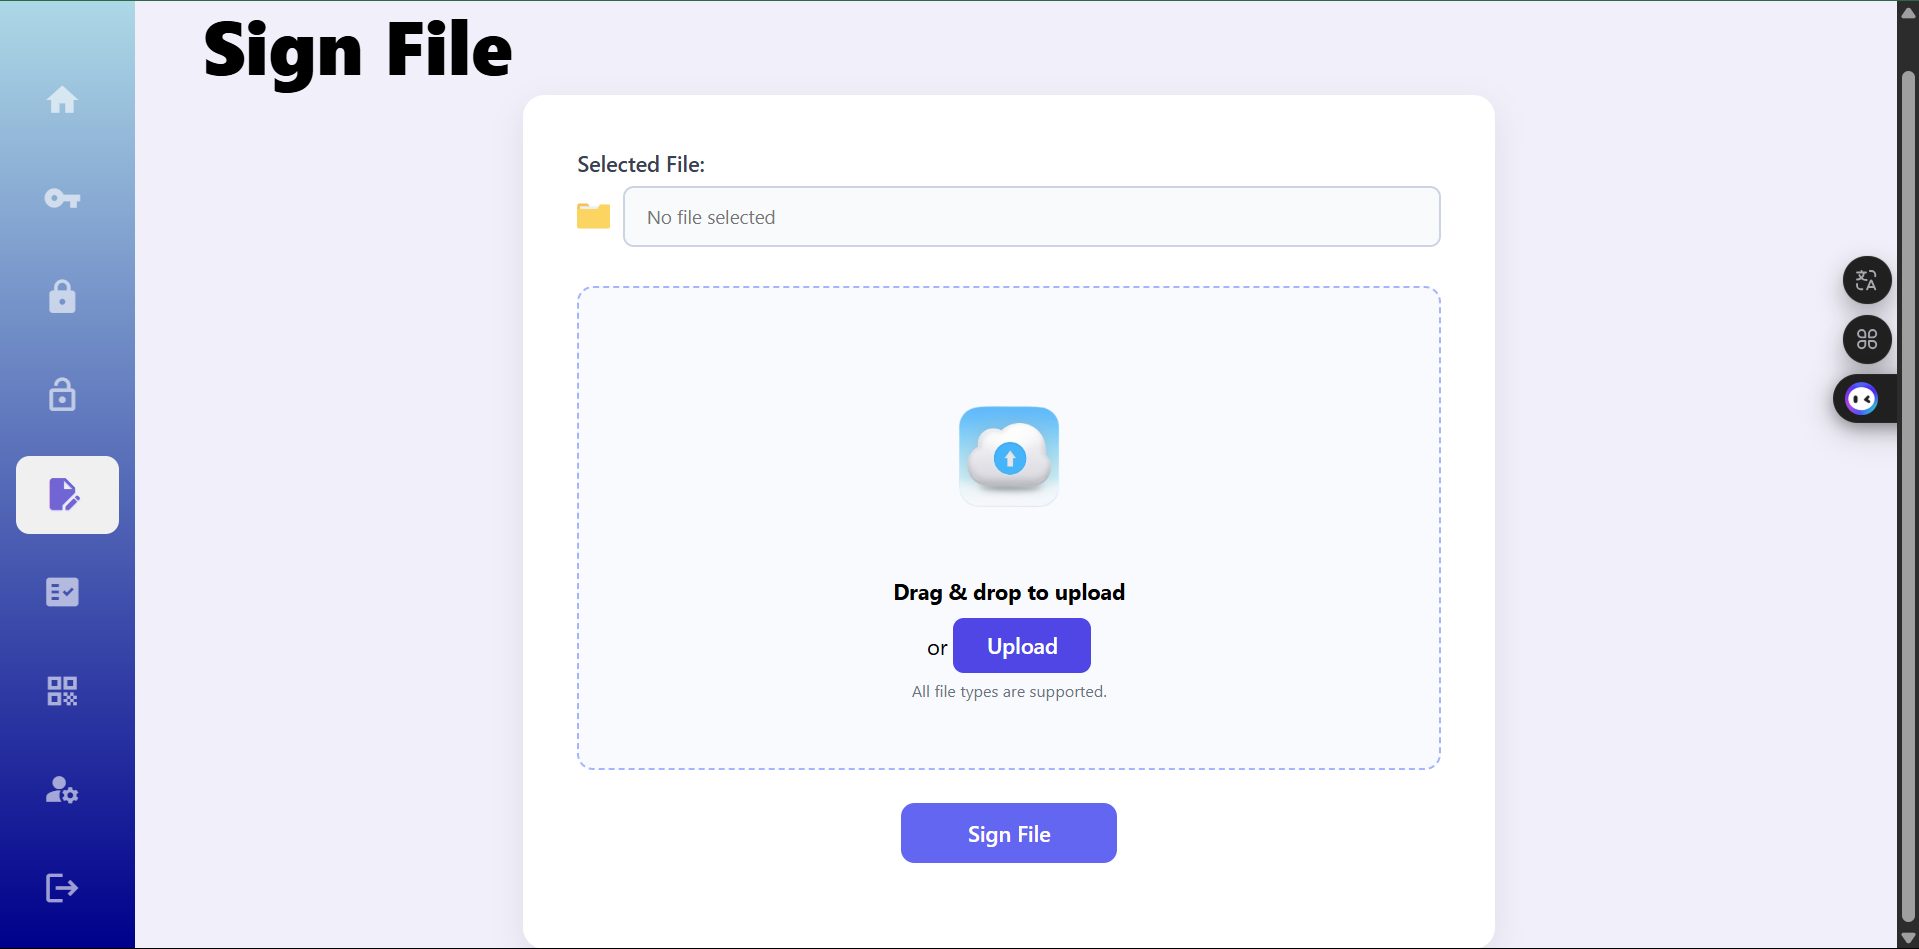
\includegraphics[width=0.85\textwidth]{img/8_sign/8_sign_form.png}
    \caption{Giao diện ký số và nút tải file chữ ký}
\end{figure}

\subsubsection*{Quy trình thực hiện}

\begin{description}
    \item[\textbf{Bước 1 - Frontend:}]
    Người dùng chọn file và submit form. File được gửi lên server bằng \texttt{fetch()} qua \texttt{FormData}:
    \begin{itemize}
        \item Gửi POST đến \texttt{/utils/sign\_file}
        \item Header \texttt{Content-Type} là \texttt{multipart/form-data}
        \item Khi server trả về file \texttt{.sig}, frontend tạo link download động và tự động tải về
    \end{itemize}

    \begin{figure}[H]
        \centering
        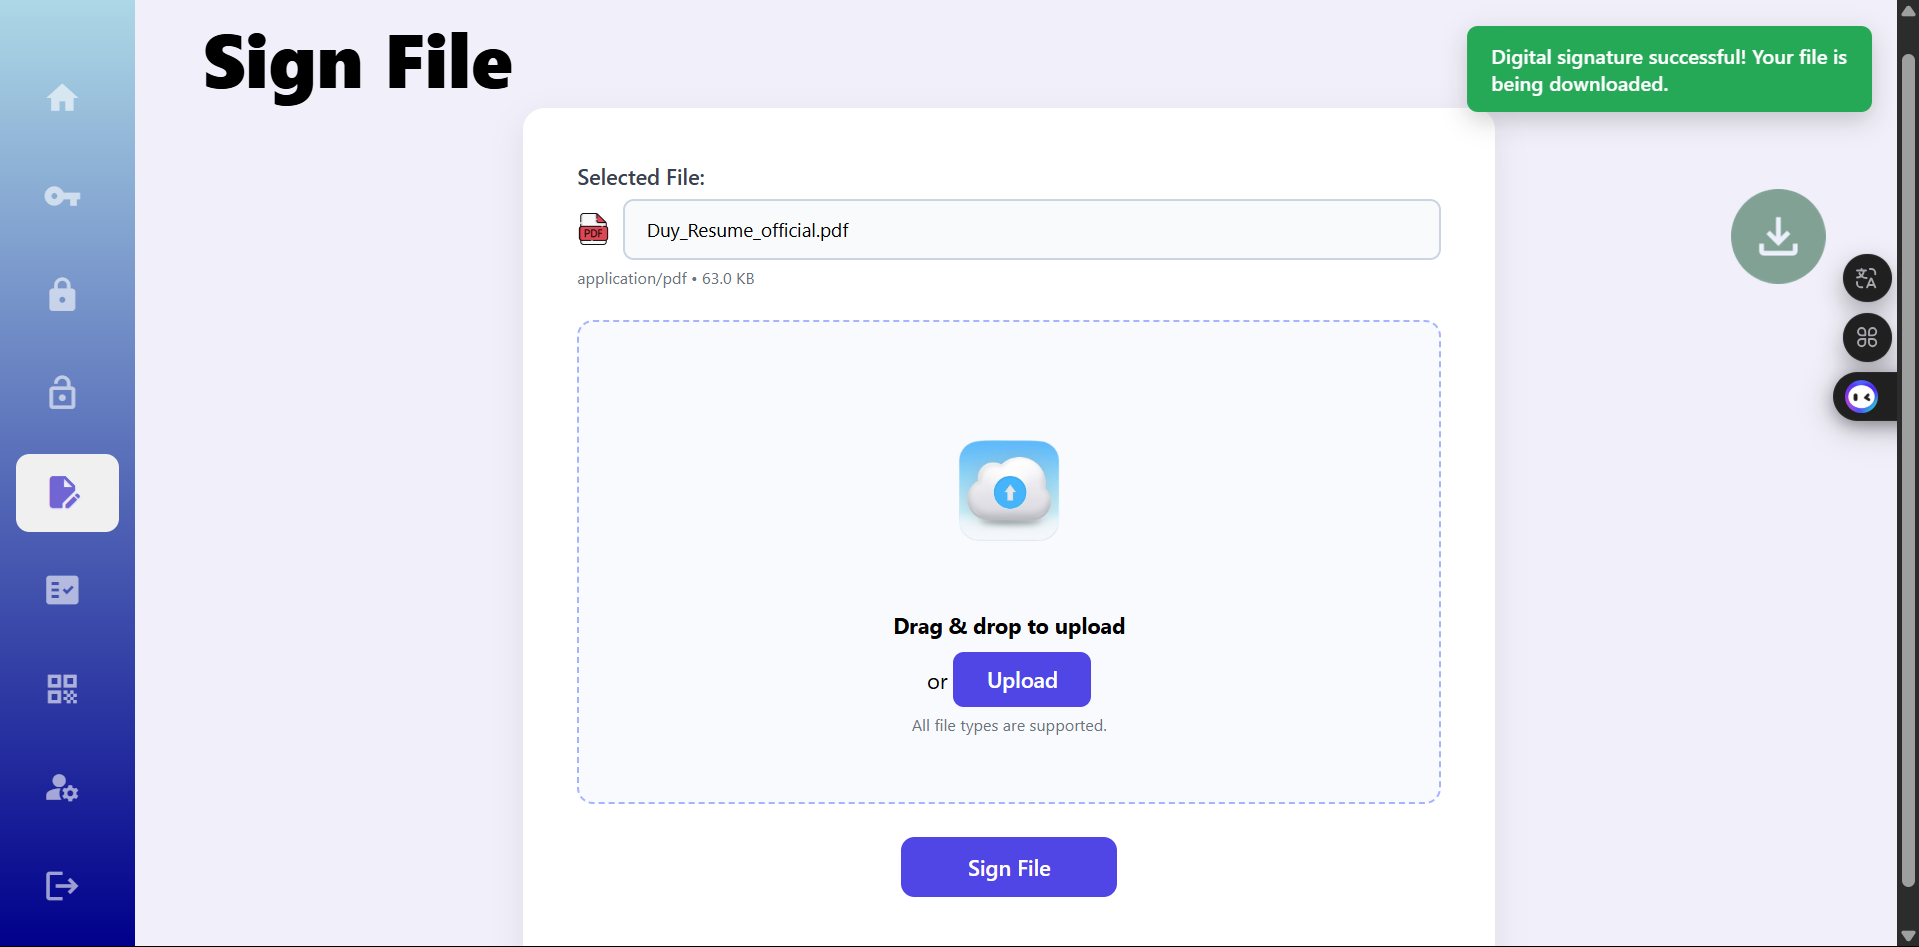
\includegraphics[width=0.85\textwidth]{img/8_sign/8_sign_success.png}
        \caption{Ký số thành công}
    \end{figure}

    \begin{figure}[H]
        \centering
        
\includegraphics[width=0.85\textwidth]{img/8_sign/8_sign_down.png}
        \caption{Tự động tải file chữ ký}
    \end{figure}

    \item[\textbf{Bước 2 - Flask Route:}]
    Route \texttt{/sign\_file} kiểm tra:
    \begin{enumerate}
        \item Đã đăng nhập và có session
        \item Có passphrase trong session để giải mã khóa riêng
        \item Tìm salt người dùng $\rightarrow$ derive AES key $\rightarrow$ giải mã private key
        \item Gọi hàm \texttt{digital\_sign\_file(file, private\_key)}
        \item Trả về file \texttt{.sig} cho trình duyệt dưới dạng \texttt{application/octet-stream}
    \end{enumerate}

    \item[\textbf{Bước 3 - Xử lý ký số (Modules):}]
    Hàm \texttt{digital\_sign\_file()} thực hiện:
    \begin{enumerate}
        \item Đọc toàn bộ nội dung file $\rightarrow$ tính hash SHA-256
        \item Ký bằng \texttt{private\_key.sign(...)} sử dụng \texttt{PKCS1v15 + SHA-256}
        \item Base64 hóa chữ ký $\rightarrow$ tạo JSON \texttt{\{"filename": ..., "signature": ..., "timestamp": ...\}}
        \item Ghi file chữ ký \texttt{.sig} vào thư mục \texttt{data/signature/}
    \end{enumerate}

    \begin{figure}[H]
        \centering
        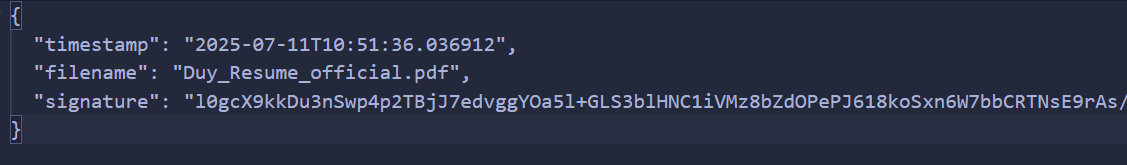
\includegraphics[width=0.85\textwidth]{img/8_sign/8_sign_json.png}
        \caption{Ghi file chữ ký}
    \end{figure}
\end{description}

\subsubsection*{Chi tiết kỹ thuật và thư viện bảo mật}

\begin{description}

    \item[\textbf{1. Ký số SHA-256 + RSA:}]
    Quá trình ký số bắt đầu bằng việc băm nội dung tập tin bằng SHA-256, sau đó dùng khóa riêng RSA để tạo chữ ký số.
    \begin{itemize}
        \item Dùng \texttt{hashlib.sha256(file\_bytes).digest()} để tính hash
        \item Dùng \codefile{cryptography.hazmat.primitives.asymmetric.rsa} để ký
        \item Padding: \codefile{PKCS1v15()}, Hash: \codefile{SHA256()}
    \end{itemize}

    \item[\textbf{2. Mã hóa và giải mã private key:}]
    Private key được bảo vệ bằng AES sử dụng passphrase người dùng. Khi cần ký, passphrase được lấy từ session để giải mã khóa.
    \begin{itemize}
        \item Private key được AES hóa bằng passphrase người dùng khi tạo khóa
        \item Để ký, passphrase được lấy từ session và dùng để giải mã khóa
    \end{itemize}

    \item[\textbf{3. Ghi log:}]
    Hệ thống ghi lại đầy đủ mọi thao tác ký dưới dạng log bảo mật – gồm cả hành động của người dùng và sự kiện nội bộ hệ thống.
    \begin{itemize}
        \item \textbf{Log người dùng:} sử dụng \texttt{log\_user\_action()} ghi lại email, hành động, trạng thái và lỗi nếu có
        \item \textbf{Log nội bộ:} \texttt{log\_internal\_event()} lưu các sự kiện kỹ thuật như “Signed filename successfully...”
    \end{itemize}

    \item[\textbf{4. Bảo mật tổng thể:}]
    Quy trình ký số đảm bảo private key không bao giờ rời khỏi server, ngăn rò rỉ khóa, đồng thời có thể truy vết mọi hoạt động.
    \begin{itemize}
        \item Tránh truyền private key về phía client – xử lý toàn bộ phía server
        \item Tất cả chữ ký lưu kèm timestamp và filename để tăng khả năng truy vết
        \item Chỉ người dùng đã đăng nhập mới được phép truy cập chức năng ký
    \end{itemize}

    \item[\textbf{5. Xử lý lỗi và báo lỗi chi tiết:}]
    Hệ thống đảm bảo mọi tình huống lỗi trong quá trình ký số đều được kiểm tra, phản hồi rõ ràng cho frontend, đồng thời ghi log đầy đủ để phục vụ giám sát bảo mật.
    \begin{itemize}
        \item Kiểm tra session: Nếu chưa đăng nhập → trả lỗi 401 với thông báo \texttt{"You must be logged in to access this page."}.
        \item Kiểm tra file đầu vào: Nếu không có file hoặc tên file rỗng → trả lỗi 400: \texttt{"No file provided."}.
        \item Kiểm tra passphrase: Nếu thiếu → trả lỗi 401: \texttt{"Passphrase not found."}.
        \item Kiểm tra lỗi phát sinh khi đọc salt, giải mã khóa riêng hoặc ký file:
        \begin{itemize}
            \item Nếu bất kỳ bước nào bị lỗi → trả lỗi 500 kèm thông báo: \texttt{"Error during digital signing: <error>"}.
            \item Toàn bộ lỗi được ghi log với \texttt{level="error"} để phục vụ phân tích.
        \end{itemize}
        \item Ghi log thất bại bằng \texttt{log\_user\_action(..., "Fail", ...)} với lý do chi tiết cho từng trường hợp.
    \end{itemize}

    \begin{figure}[H]
        \centering
        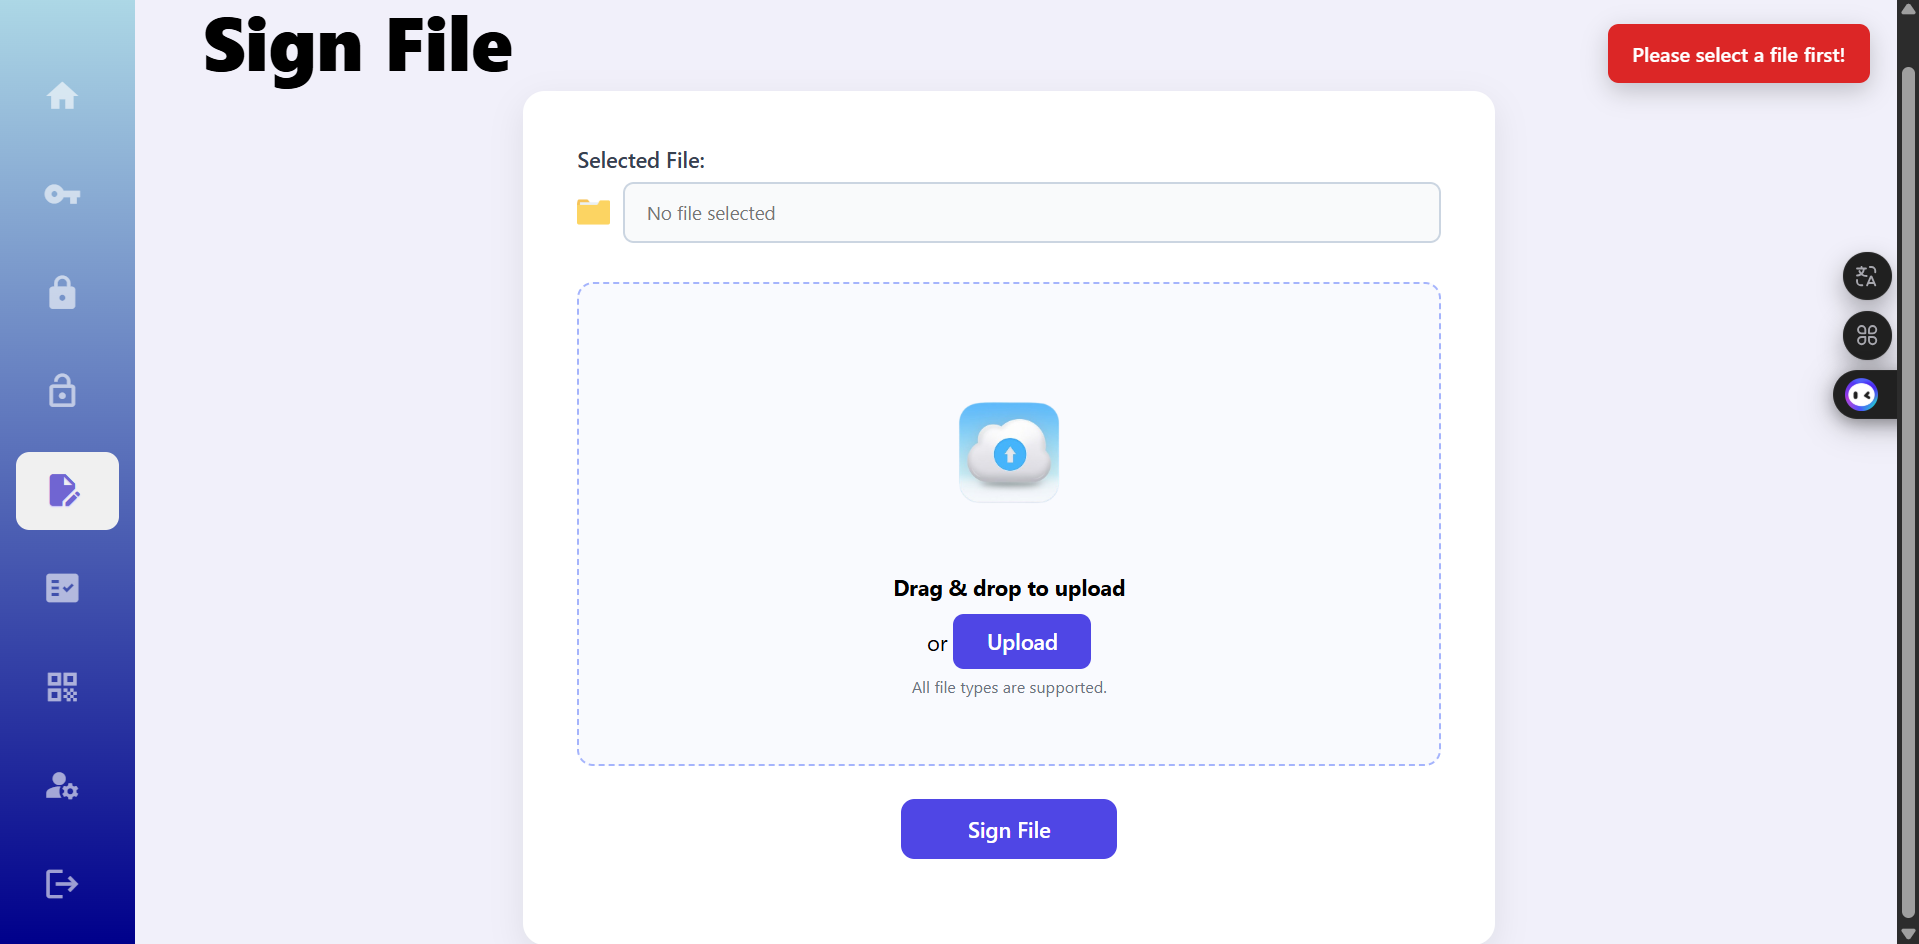
\includegraphics[width=0.85\textwidth]{img/8_sign/8_sign_fail.png}
        \caption{Báo lỗi nếu chưa chọn file}
    \end{figure}

\end{description}

